\documentclass[../report.tex]{subfiles}
\graphicspath{{\subfix{../image/}}}

\begin{document}
\subsection{Motordriver PCB}
This is a 2 layer PCB for the Motordriver. 
\begin{figure}[H]
    \centering
    \begin{subfigure}[b]{0.4\linewidth}
      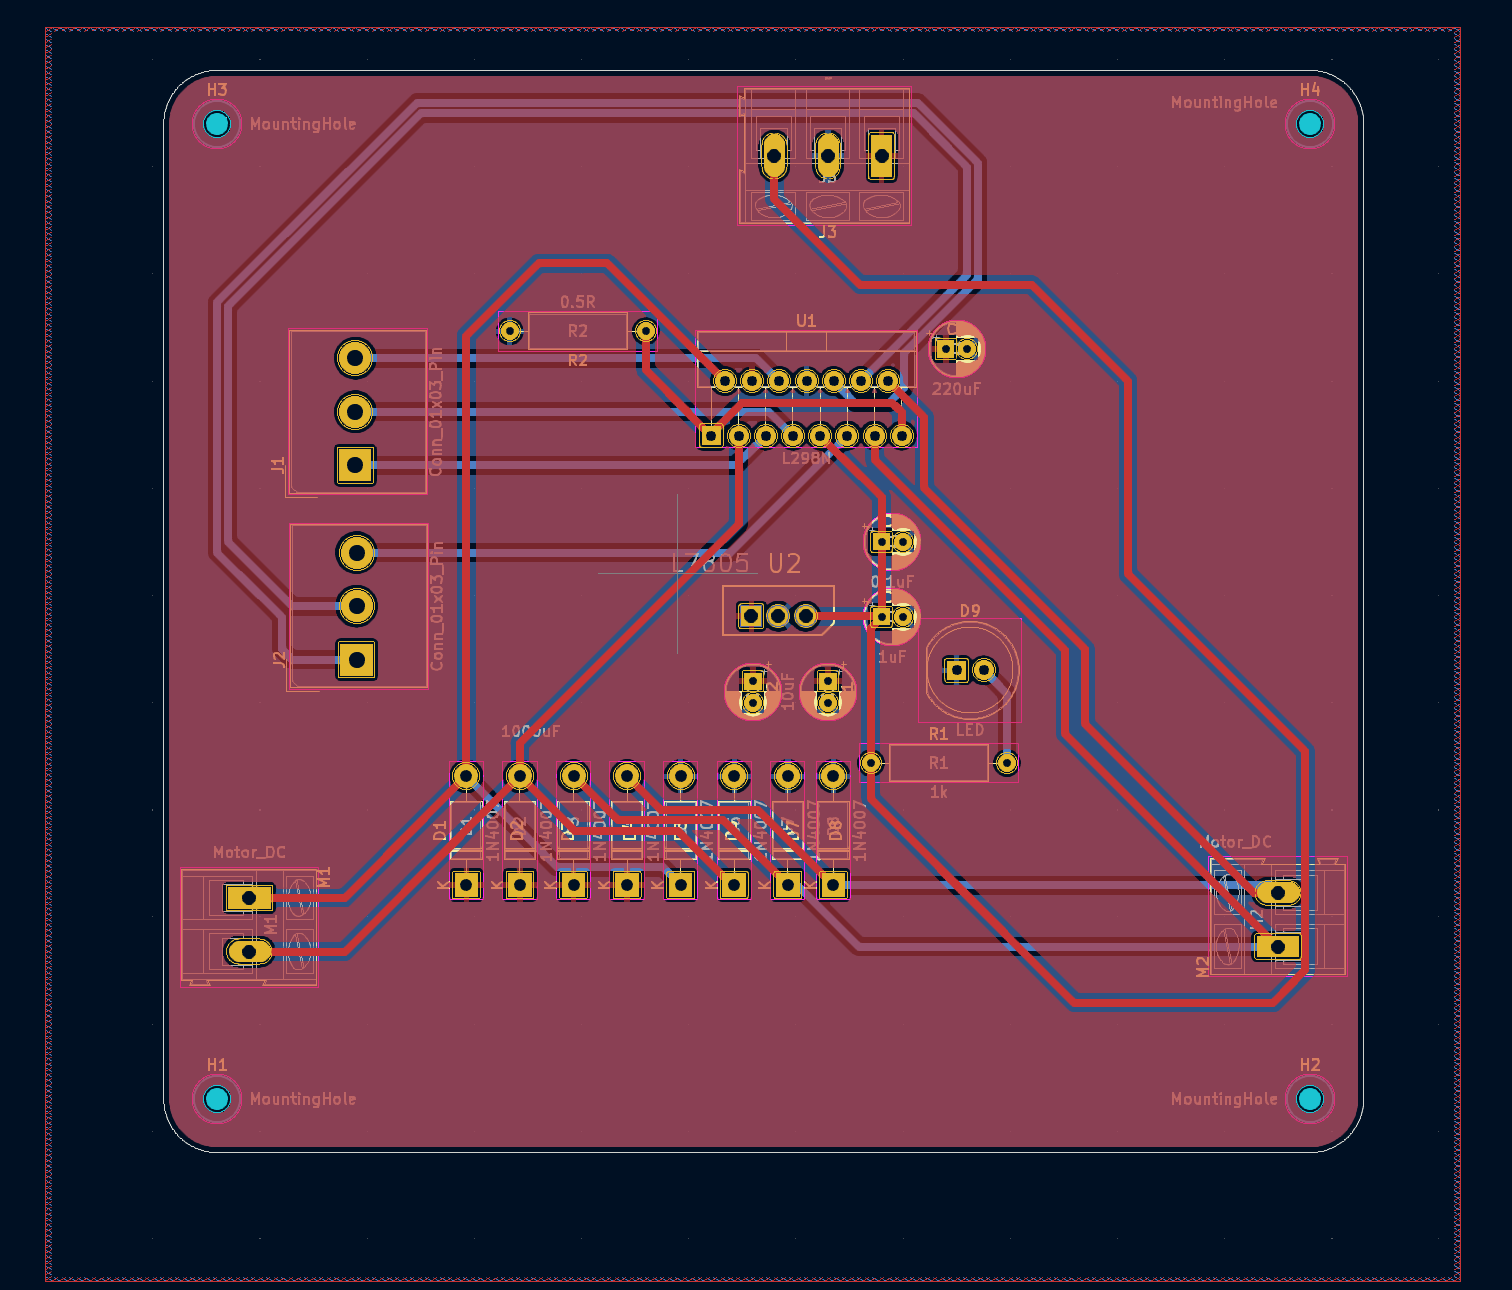
\includegraphics[width=\linewidth]{Screenshot 2023-12-14 at 16.22.46.png}
      \caption{Motordriver PCB} 
    \end{subfigure}
    \begin{subfigure}[b]{0.4\linewidth}
      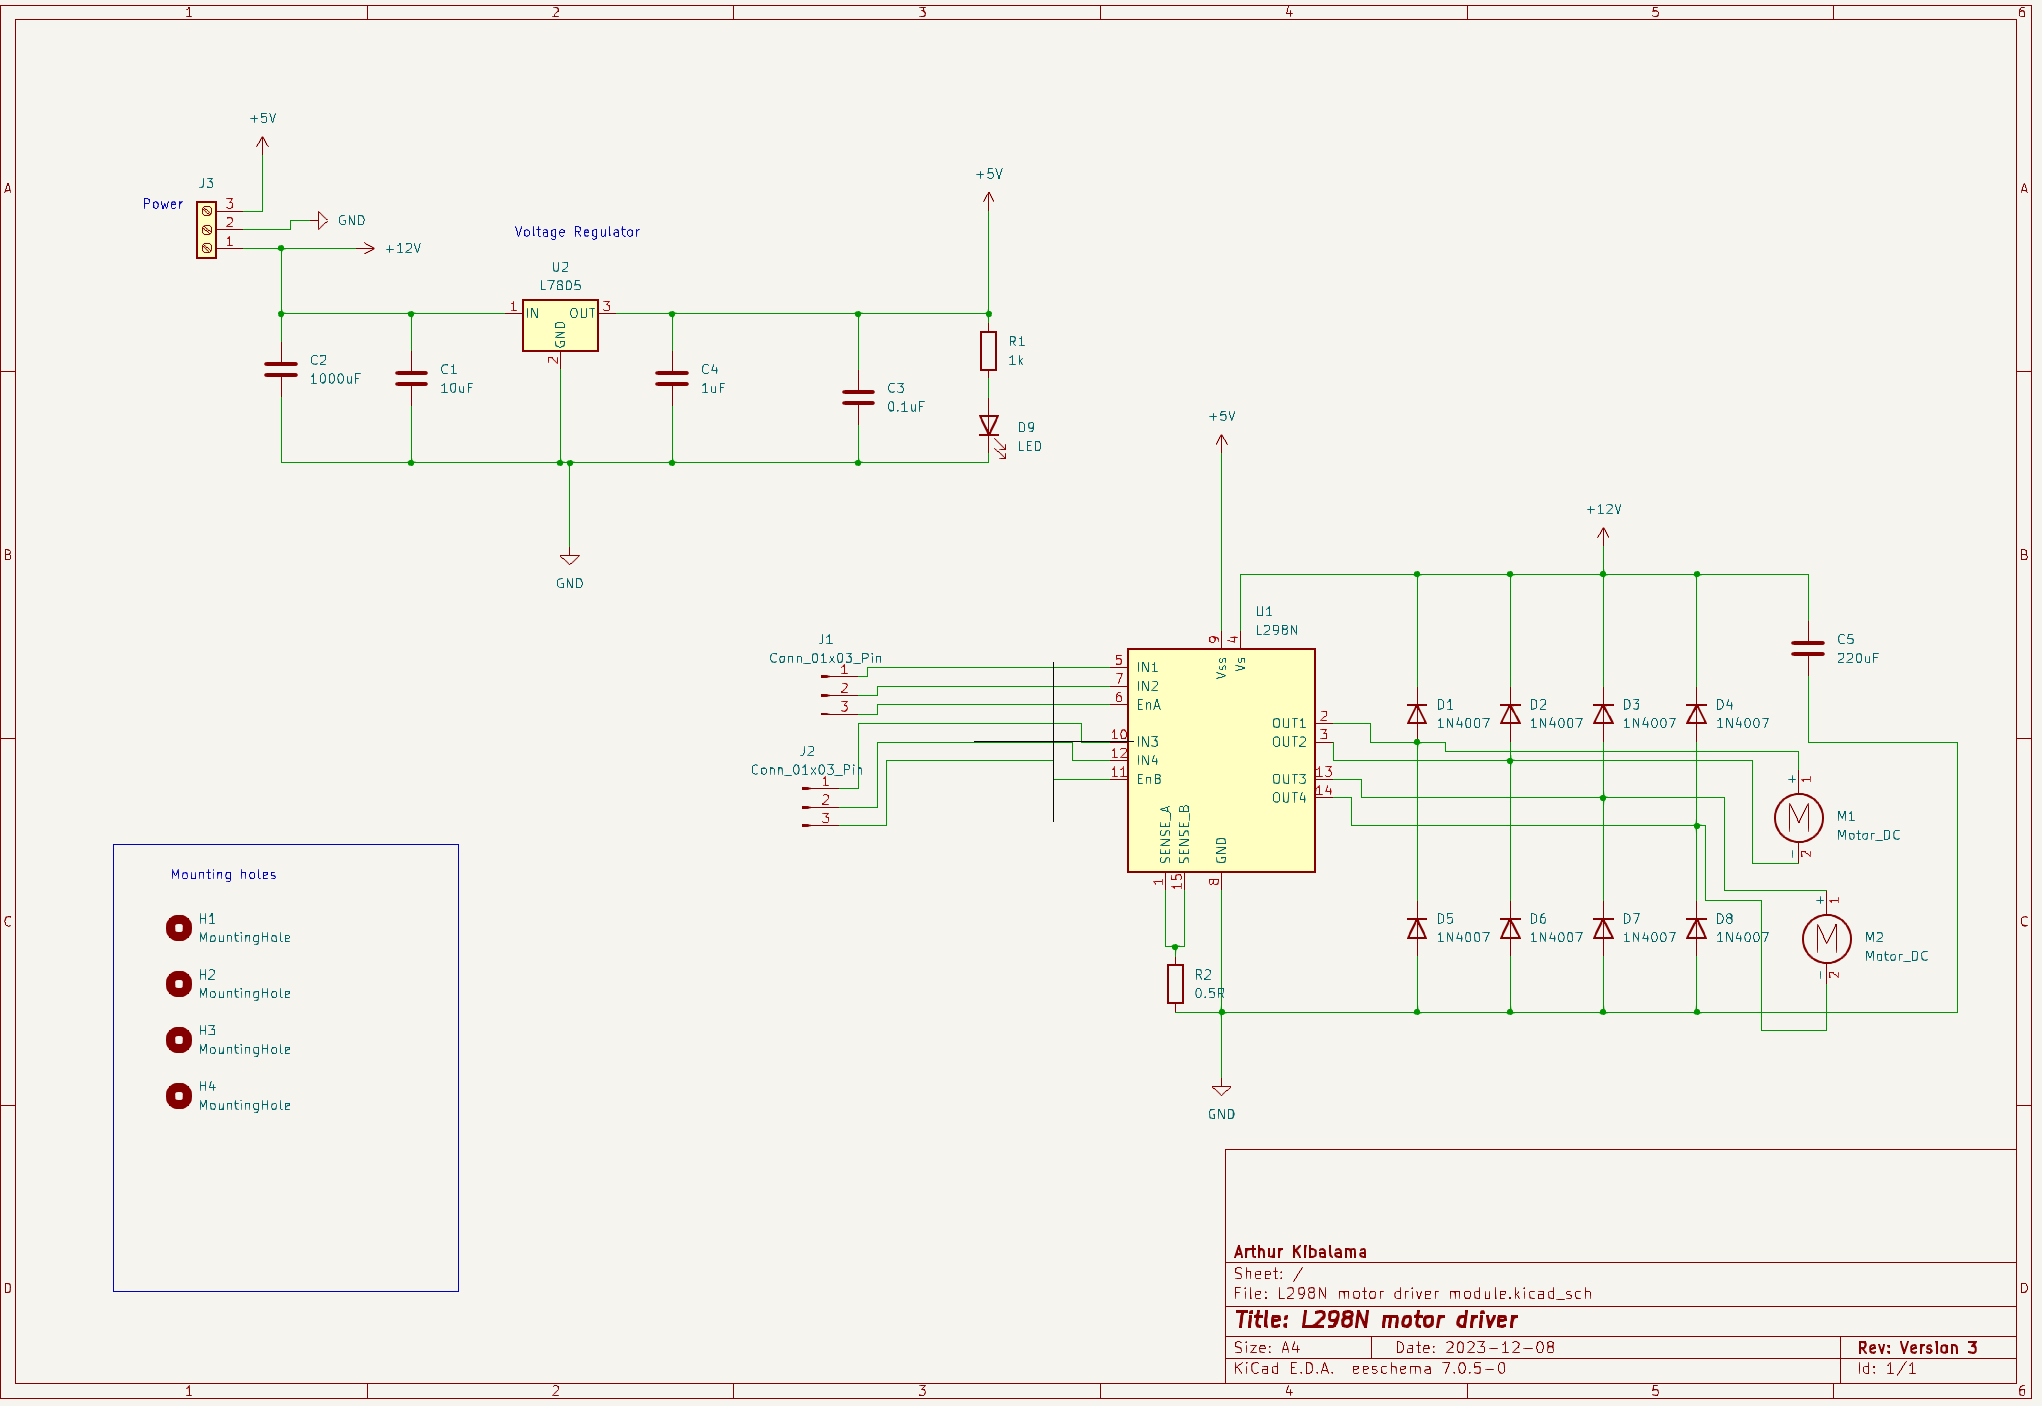
\includegraphics[width=\linewidth]{Screenshot 2023-12-14 at 16.50.36.png}
      \caption{L298n Motordriver Schematic}
    \end{subfigure}
  \end{figure}
  \subsection*{How I designed the PCB}
  \subsubsection*{Decoupling Capacitors}
  In the strictest definition, a decoupling capacitor isn't a distinct component per se, instead it characterizes a capacitor's role within an electronic circuit. 
  Its primary function is to enhance stability on the power supply plane by mitigating voltage fluctuations. In any design involving semiconductor ICs, the inclusion of decoupling capacitors is imperative. This is because the voltage supplied to the components deviates significantly from the ideal scenario. Unlike the theoretical perfectly steady line, real-world voltage readings exhibit fluctuations, even with a meticulously clean power supply.
  The decoupling capacitor operates as a reservoir, contributing to voltage stabilization through two key mechanisms. First, it absorbs excess charges when the voltage surpasses the rated value. Simultaneously, it releases stored charges when the voltage decreases, ensuring a consistently stable power supply.
  Typically, a combination of at least two capacitors with different values is employed to stabilize the voltage supplied to a component's VDD pin. A capacitor around 10 uF serves as a substantial buffer to smooth out low-frequency fluctuations, while a smaller capacitor of approximately 100 nF addresses high-frequency changes in voltage. 
\end{document}